\pdfminorversion=5 % To enforce 1.5 version of PDF

% Preamble
% =============================================================
\documentclass[xcolor=table]{beamer}        % Just Slides
%\documentclass[xcolor=table,notes]{beamer} % Slides and Notes


% Encoding
% =============================================================
\usepackage[english]{babel}
\usepackage[latin1]{inputenc}


% Beamer Class Template Settings
% =============================================================
\usetheme[compress]{Dresden}
\setbeamercovered{transparent}
\usefonttheme[onlysmall]{structurebold}
\beamertemplatenavigationsymbolsempty
\useinnertheme[shadow=true]{rounded}
\usefonttheme[onlymath]{serif}


% Packages
% =============================================================
\usepackage{color}
\usepackage{colortbl}
\usepackage{ziffer}
\usepackage{amsmath,amsfonts,amssymb}
\usepackage{etex}
\usepackage[absolute,overlay]{textpos}
\usepackage{framed}
\usepackage{media9}
\usepackage{hyperref}

\hypersetup{
pdfstartview={Fit},
bookmarks=True,
pdftitle={Git Workshop},
pdfauthor={Nicolas Guarin-Zapata, Cyrus Vandrevala},
pdfsubject={Lectures},
pdfkeywords={Version control, Scientific Computing}
}


% Definitions
% =============================================================
\setlength{\TPVertModule}{\paperheight}
\setlength{\TPHorizModule}{\paperwidth}
\setlength{\TPHorizModule}{\paperwidth}\setlength{\TPVertModule}{\paperheight}

\setbeamercolor{footlinecolor}{bg=RUBgrau,fg=RUBblau}

% Footline Information
\setbeamertemplate{footline}{
  \begin{beamercolorbox}[sep=1em, wd=\paperwidth,leftskip=0.4cm,rightskip=0.4cm]{footlinecolor}
  \mbox{
    \begin{minipage}{0.2\paperwidth}
	  
\includegraphics[width=0.1\paperwidth]{img/Purdue-logo-BW2.pdf}
	\end{minipage}
	\begin{minipage}{0.6\paperwidth}
	  \begin{center}
	    Git Workshop
	  \end{center}
	\end{minipage}
	\begin{minipage}{0.2\paperwidth}
	  \scriptsize{\insertframenumber}
	\end{minipage}}
  \end{beamercolorbox}
}


% Colors
% =============================================================
\definecolor{RUBgrau}   {HTML}{e6e4e4}
\definecolor{RUBblau}   {HTML}{003560}
\definecolor{RUBgruen}  {HTML}{94c11c}
\definecolor{middlegray}{rgb} {0.5,0.5,0.5}
\definecolor{lightgray} {rgb} {0.97,0.97,0.97}
\definecolor{tablegray} {rgb} {0.85,0.85,0.85}
\definecolor{white}     {rgb} {1.0,1.0,1.0}
\definecolor{orange}    {rgb} {0.8,0.3,0.3}
\definecolor{yac}       {rgb} {0.6,0.6,0.1}
\definecolor{red}       {rgb} {1.0,0,0}
\definecolor{green}     {rgb} {0.0,1.0,0.0}
\definecolor{black}     {rgb} {0,0,0}
\definecolor{blue}      {rgb} {0,0,1.0}
\definecolor{lightblue} {rgb} {0.5,0.9,1.0}


% Beamer Class Color Settings
% =============================================================
\setbeamercolor{block body example}{bg=RUBgrau}
\setbeamercolor{block title example}{bg=RUBblau,fg=white}
\setbeamercolor{block body alerted}{bg=RUBgrau}
\setbeamercolor{block title alerted}{bg=red,fg=black}

\setbeamercolor{section in head/foot}{fg=white, bg=RUBblau}
\setbeamercolor{subsection in head/foot}{fg=black, bg=white}
\setbeamercolor{block title}{fg=RUBblau}
\setbeamercolor{section in toc}{fg=RUBblau}
\setbeamercolor{section}{fg=RUBblau}
\setbeamercolor{item}{fg=RUBblau}
\setbeamercolor{frametitle}{fg=RUBblau,bg=RUBgrau}
\setbeamercolor{framesubetitle}{fg=black}
\setbeamercolor{title}{fg=RUBblau,bg=RUBgrau}
\setbeamercolor{titlelike}{bg=RUBblau}

\setbeamercolor{palette sidebar primary}{use=normal text,fg=normal text.fg}
\setbeamercolor{palette sidebar quaternary}{use=structure,fg=structure.fg}
\setbeamercolor{palette sidebar secondary}{use=structure,fg=structure.fg}
\setbeamercolor{palette sidebar tertiary}{use=normal text,fg=normal text.fg}

\setbeamercolor{section in sidebar}{fg=RUBgrau}
\setbeamercolor{section in sidebar shaded}{fg=RUBgrau}
\setbeamercolor{separation line}{}
\setbeamercolor{sidebar}{bg=RUBgrau}
\setbeamercolor{sidebar}{parent=palette primary}


% Title Page Customization
% =============================================================
\setbeamertemplate{title page}{
  \vspace{0.25cm}
  \begin{columns}
    \column{.6\textwidth}
      \insertsubtitle\\
	  \vspace{0.5cm}
	  {\usebeamerfont{title}\usebeamercolor[fg]{title}\inserttitle}\\
	  \vspace{0.5cm}
	  \insertauthor\\
	  \vspace{2mm}
	  \insertdate
	  \vfill
    \column{.4\textwidth}
	\begin{center}
	  
\includegraphics[width=0.9\textwidth]{img/Git-logo}\\
	  \vspace{3mm}
	  
\includegraphics[width=0.9\textwidth]{img/github_logos/GitHub_Logo}\\
	  \vspace{3mm}
	  
\includegraphics[width=0.9\textwidth]{img/Purdue-logo-BW2}
    \end{center}
  \end{columns}
}


%%%%%%%%%%%%%%%%%%%%%%%%%%%%

% TITLE SLIDE PARAMETERS
\title{Version Control Workshop: Git and GitHub}
\subtitle{Day 1}
\institute{Purdue University}
\author[AUTHOR]{\scriptsize{Cyrus Vandrevala $^1$\\Nicol\'as Guar\'in-Zapata$^2$}\\
\tiny{$^1$ Physics Department\\ $^2$ Civil Engineering Department}}
\date{October 30-31, 2014}

%%%%%%%%%%%%%%%%%%%%%%%%%%%%

\begin{document}

% TITLE SLIDES
\begin{frame}[plain]
\titlepage
\end{frame}

\begin{frame}
\frametitle{\large{Overview}}
\tableofcontents
\end{frame}

\begin{frame}
\frametitle{\large{We Encourage Participation!}}
\begin{itemize}
\item Post Questions That You Might Have in the Repo
\item Recommend Other Sources That You Found Useful
\item Remember, We Do Not Know Everything!
\end{itemize}
\end{frame}

%%%%%%%%%%%%%%%%%%%%%%%%%%%%

% CONTENT
% ======================================= %
% INTRODUCTION TO VERSION CONTROL
% ======================================= %

\section[Introduction]{Introduction to Version Control}

% WHAT IS VERSION CONTROL?
\begin{frame}
\frametitle{\large{What is Version Control?}}
Version control is a system that records changes to a file or set of files over time so that you can recall specific versions later. \\
\vspace{3mm}
- \emph{Pro Git}, Chapter 1
\end{frame}
\note{}

\begin{frame}
\frametitle{\large{What is Version Control?}}
It allows you to revert files back to a previous state, revert the entire project back to a previous state, compare changes over time, see who last modified something that might be causing a problem, who introduced an issue and when, and more. \\
\vspace{3mm}
- \emph{Pro Git}, Chapter 1
\end{frame}
\note[itemize]{
\item One of the first major version control systems was the Revision Control System (RCS). It was released by Walter F. Tichy while he was at Purdue University (RCS: A System for Version Control).
}

% WHY IS VERSION CONTROL IMPORTANT?
\begin{frame}
\frametitle{\large{Why is Version Control Important?}}
\begin{enumerate}
\item Keep Track of Code History
\pause
\item Concurrent Teamwork
\pause
\item Coordinate Coding Environments
\pause
\item Due Diligence Checks
\pause
\item Share Code
\end{enumerate}
\pause
\vspace{5mm}
Everybody Should Use Version Control!
\end{frame}
\note{}

% WHAT OPTIONS ARE AVAILABLE? (part 1)
\begin{frame}
\frametitle{\large{What Options Are Available?}}
\textbf{Option \#1: Client-Server Version Control Systems}
\vspace{8mm}
\begin{columns}[c]
\column{2in}
{\small \textbf{Advantages}}
\begin{enumerate}
\small
\item A Single Admin Keeps Track of the Project
\item There is a Single Master Version of the Code
\item It is Relatively Easy to Learn
\end{enumerate}
\column{2in}
{\small \textbf{Disadvantages} }
\begin{enumerate}
\small
\item There Is Only One Admin/Server
\item You Need a Network Connection to Work
\item Operations Can Be Slow
\end{enumerate}
\end{columns}
\vspace{5mm}
{\small Examples include Concurrent Versions System (CVS) and Subversion (SVN).}
\end{frame}
\note{}

% WHAT OPTIONS ARE AVAILABLE? (part 2)
\begin{frame}
\frametitle{\large{What Options Are Available?}}
\textbf{Option \#2: Distributed Version Control Systems}
\vspace{8mm}
\begin{columns}[c]
\column{2in}
{\small \textbf{Advantages}}
\begin{enumerate}
\small
\item You Don't Need a Network Connection
\item Multiple Coding Environments
\item It Encourages Collaboration and Modularity
\end{enumerate}
\column{2in}
{\small \textbf{Disadvantages}}
\begin{enumerate}
\small
\item Can Be Difficult to Learn
\item Teams Need to Talk About Conventions
\item It is Really Easy To Create Unorganized Code
\end{enumerate}
\end{columns}
\vspace{5mm}
{\small Examples include Git, Mercurial, and Bazaar.}
\end{frame}
\note{}

% WHY GIT AND GITHUB? (part 1)
\begin{frame}
\frametitle{\large{Why Git and GitHub?}}
\begin{enumerate}
\item It Keeps Track of Detailed Metadata (More Than Others)
\item Branching is Encouraged (Which Modularizes Development)
\item Most Operations in Git are Local (Which Increases Speed)
\item GitHub Has a Great Social Community
\end{enumerate}
\end{frame}
\note{}

% WHY GIT AND GITHUB? (part 2)
\begin{frame}
\frametitle{\large{Why Git and GitHub?}}
Full Disclosure...
\begin{enumerate}
\item It Isn't the Best for Binary Files
\item GitHub Distinguishes Between Public and Private Repos
\end{enumerate}
\end{frame}
\note{}

% ======================================= %
% WORKFLOW IN COMPUTATIONAL SCIENCE
% ======================================= %

\section[Work Flow]{Work Flow in Computational Science}

\begin{frame}
\frametitle{\large{Version Control in Academia}}
\begin{enumerate}
\item It Creates Reproducible Research
\item It Helps Train New Group Members
\item It Encourages Collaboration
\item It Encourages Good Code Practices
\end{enumerate}
\end{frame}
\note{}

\begin{frame}
\frametitle{\large{Reproducible Research}}
Purdue is already taking action in this subject:
\begin{itemize}
\item  Purdue University Research Repository (PURR): \url{https://purr.purdue.edu/}
\end{itemize}
\vspace{3mm}
We can create a DOI for a GitHub repository using \texttt{zenodo.org}:
\begin{itemize}
\item \small \url{https://guides.github.com/activities/citable-code/}
\end{itemize}
\end{frame}
\note{}

\begin{frame}
\frametitle{\large{Reproducible Research}}
\begin{columns}[c]
\column{2in}
A Cool Example:

\vspace{3mm}
\emph{\small Silverberg, Jesse L., et al. ``Collective motion of humans in mosh and circle pits at heavy metal concerts." Physical review letters 110.22 (2013): 228701.}
\vspace{5mm}

Repo: \url{https://github.com/mattbierbaum/moshpits}
\column{2in}
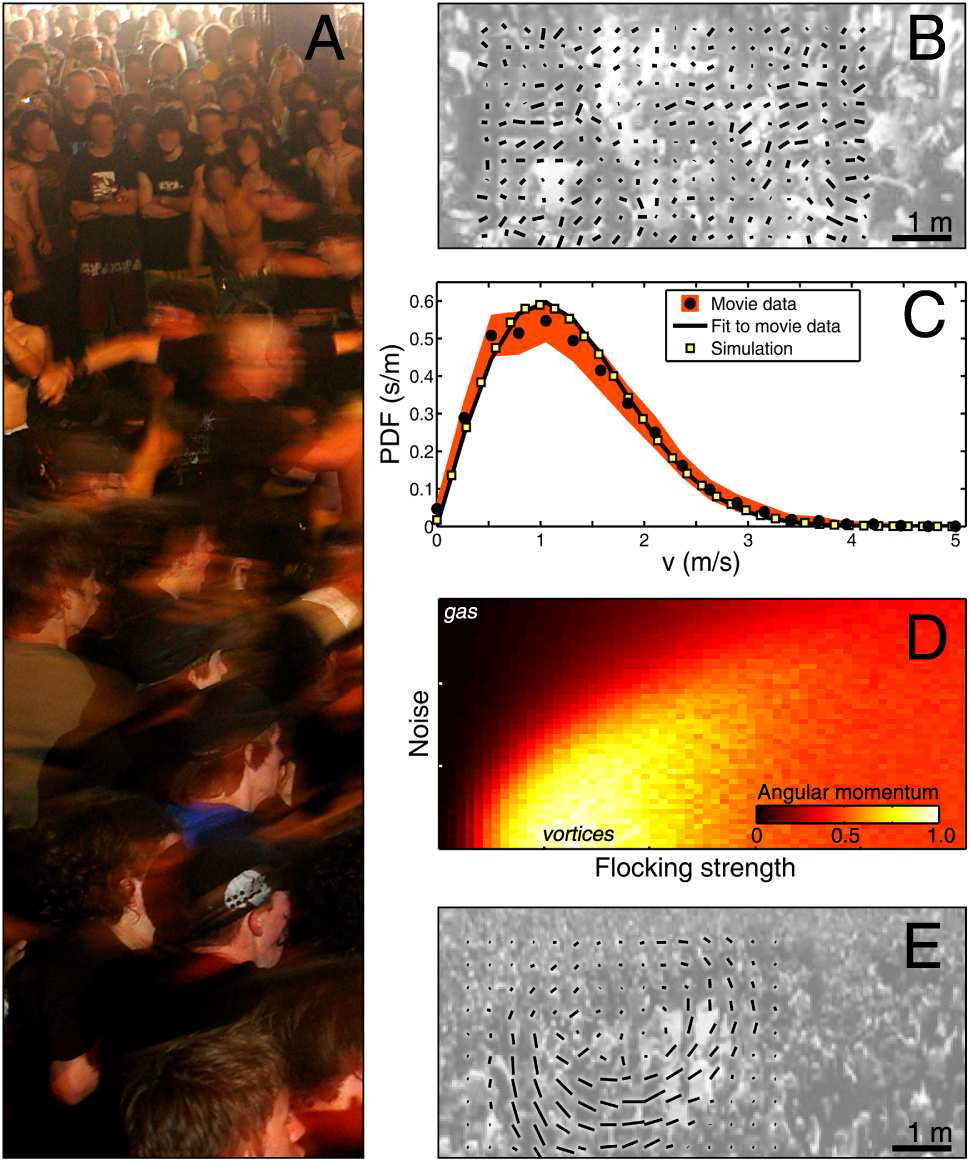
\includegraphics[width=2in]{img/mosh_physics.png}
\end{columns}

\end{frame}
\note{}

\begin{frame}
\frametitle{\large{Some Useful Skills}}
Some Useful Skills That You Should Learn Are:
\begin{enumerate}
\item Bash
\item Markdown
\item Vim and/or Emacs
\end{enumerate}
\end{frame}
\note{}
% ======================================= %
% SETTING UP GIT
% ======================================= %

\section[Setting Up Git]{Setting Up Git On Your Machine}

\begin{frame}
\frametitle{\large{Setting Up Git - Linux}}
You can use the package management tool that comes with your distribution (use sudo):
\begin{enumerate}
\item yum install git
\item apt-get install git
\end{enumerate}
\end{frame}
\note{}

\begin{frame}
\frametitle{\large{Setting Up Git - Mac}}
There are three main ways to install Git:
\begin{enumerate}
\item Install the Xcode Command Line Tools and Type ``git'' Into the Terminal
\item Binary Installer: \href{http://git-scm.com/download/mac}{http://git-scm.com/download/mac}
\item Git/GitHub GUI: \href{https://mac.github.com/}{https://mac.github.com/}
\end{enumerate}
\end{frame}
\note[itemize]{
\item The GUI only implements a subset of the full Git functionality, so it is best to learn how to use the command line.
}

\begin{frame}
\frametitle{\large{Setting Up Git - Windows}}
There are three main ways to install Git:
\begin{enumerate}
\item Binary Installer: \href{http://git-scm.com/download/win}{http://git-scm.com/download/win}
\item msysGit: \href{http://msysgit.github.io/}{http://msysgit.github.io/}
\item Git/GitHub GUI: \href{https://windows.github.com/}{https://windows.github.com/}
\end{enumerate}
\end{frame}
\note[itemize]{
\item The GUI only implements a subset of the full Git functionality, so it is best to learn how to use the command line.
}

\begin{frame}
\frametitle{\large{Setting Up Git - Installing From Source}}
You can also install GitHub from source. See the Git website for full instructions on how to do that.
\end{frame}
\note[itemize]{
\item http://git-scm.com/
}

\begin{frame}
\frametitle{\large{Setting Up Git - Config File}}
Git stores user information in \emph{/etc/gitconfig}, \emph{~/.gitconfig}, and \emph{/your-project/.git/config}. To set up your information: \\
\begin{itemize}
\item \emph{git config -{}-global user.name ``Cyrus Vandrevala''}
\item \emph{git config -{}-global user.email cyrus.vandrevala@gmail.com}
\item \emph{git config -{}-global core.editor vim}
\end{itemize}
\end{frame}
\note[itemize]{
\item http://git-scm.com/
}

\begin{frame}
\frametitle{\large{Setting Up Git - Config File}}
You can double check the information you entered by using: \\
\begin{itemize}
\item \emph{git config -{}-list}
\end{itemize}
\end{frame}
\note[itemize]{
\item http://git-scm.com/
}

\begin{frame}
\frametitle{\large{Setting Up a New Git Repo}}
\begin{enumerate}
\item Create a New Directory (mkdir my-awesome-directory)
\item Navigate Into the Directory (cd my-awesome-directory)
\item Initialize the Directory (git init)
\end{enumerate}
\vspace{5mm}
The git init command creates a hidden directory called .git that contains all of the metadata for the project. \emph{You should never change anything in .git directly!}
\end{frame}
\note{}

\begin{frame}
\frametitle{\large{Retrieving an Existing Git Repo}}
\begin{enumerate}
\item Navigate to the Directory Where You Want to Store the Project
\item \emph{git clone https://mydirectory.com/}
\end{enumerate}
\vspace{5mm}
\begin{itemize}
\item Git supports many transfer protocols (including SSH)
\item Remember, you are creating a standalone copy of the entire project.
\end{itemize}
\end{frame}
\note{}
% ======================================= %
% BASIC GIT WORK FLOW
% ======================================= %

\section[Basic Git]{Basic Git Work Flow}

\begin{frame}
\frametitle{\large The Basic Git Work Flow}
\begin{enumerate}
\item Synchronize Your Repo (git pull)
\item Make Changes to Your Code
\item Stage Changes for Commit (git add)
\item Commit Changes Locally (git commit)
\item Push Changes to Origin (git push)
\end{enumerate}
\end{frame}
\note{This is a note.}
% ======================================= %
% BRANCHING
% ======================================= %

\section[Branching]{Git Branches}

\begin{frame}
\frametitle{\large What is Branching?}
\begin{itemize}
\item Pretty much every version control system has some form of branching. This means that you diverge from the main line of development and continue to do work without changing the main line.
\pause
\item Usually this is an expensive process because you have to copy all of the source code in the directory into a new branch.
\pause
\item However, branching is where git truly shines. The git branch is extremely lightweight. This encourages branching in order to add new features.
\end{itemize}
\end{frame}

\begin{frame}
\frametitle{\large How Does Branching Work?}
\begin{center}
Let's look at a couple of examples from Pro Git (2nd Edition). \\
This book is licensed under the Creative Commons Attribution Non-Commercial Share Alike 3.0 License.
\end{center}
\end{frame}

\begin{frame}
\frametitle{\large How Does Branching Work?}
\begin{center}
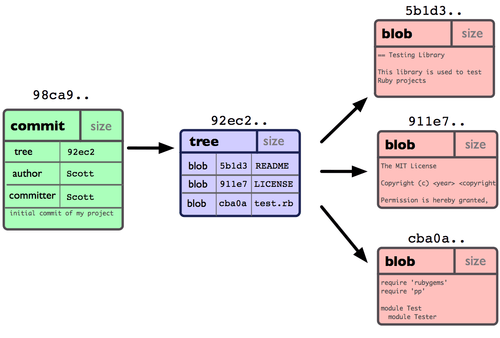
\includegraphics[width=0.7\textwidth]{img/branching_images/fig1.png}
\end{center}
\end{frame}

\begin{frame}
\frametitle{\large How Does Branching Work?}
\begin{center}
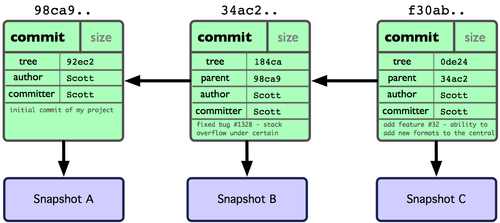
\includegraphics[width=0.7\textwidth]{img/branching_images/fig2.png}
\end{center}
\end{frame}

\begin{frame}
\frametitle{\large How Does Branching Work?}
\begin{center}
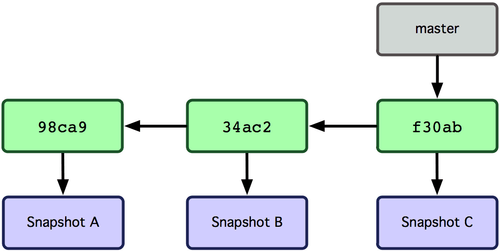
\includegraphics[width=0.7\textwidth]{img/branching_images/fig3.png}
\end{center}
\end{frame}

\begin{frame}
\frametitle{\large How Does Branching Work?}
\begin{center}
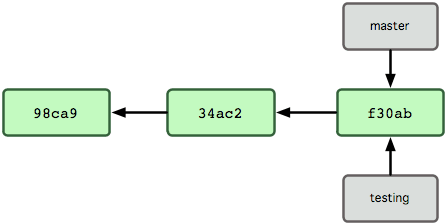
\includegraphics[width=0.7\textwidth]{img/branching_images/fig4.png}
\end{center}
\end{frame}

\begin{frame}
\frametitle{\large How Does Branching Work?}
\begin{center}
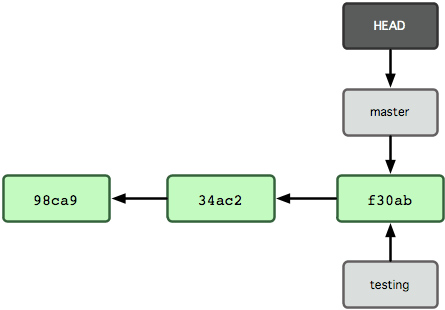
\includegraphics[width=0.7\textwidth]{img/branching_images/fig5.png}
\end{center}
\end{frame}

\begin{frame}
\frametitle{\large How Does Branching Work?}
\begin{center}
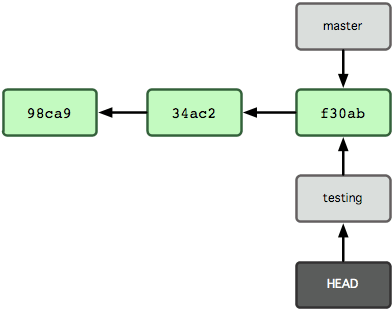
\includegraphics[width=0.7\textwidth]{img/branching_images/fig6.png}
\end{center}
\end{frame}

\begin{frame}
\frametitle{\large How Does Branching Work?}
\begin{center}
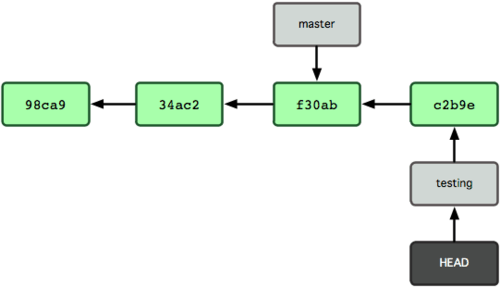
\includegraphics[width=0.7\textwidth]{img/branching_images/fig7.png}
\end{center}
\end{frame}

\begin{frame}
\frametitle{\large How Does Branching Work?}
\begin{center}
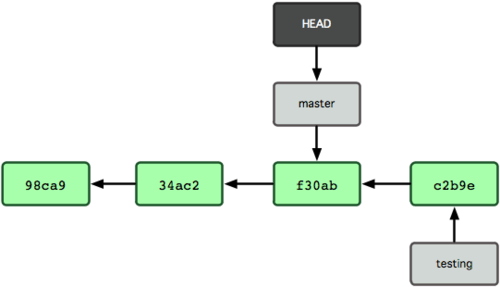
\includegraphics[width=0.7\textwidth]{img/branching_images/fig8.png}
\end{center}
\end{frame}

\begin{frame}
\frametitle{\large How Does Branching Work?}
\begin{center}
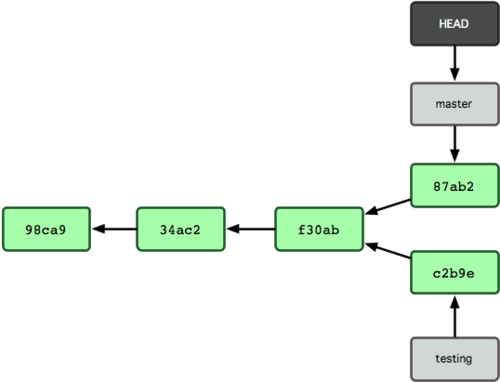
\includegraphics[width=0.7\textwidth]{img/branching_images/fig9.png}
\end{center}
\end{frame}
% ======================================= %
% DELETING FILES
% ======================================= %

\section[Deleting]{Git Delete Commands}

\begin{frame}
\frametitle{\large Delete a File (rm vs. git rm)}
\end{frame}
% ======================================= %
% GIT AND GITHUB
% ======================================= %

\section[GitHub]{Combining Git With GitHub}

\begin{frame}
\frametitle{Public vs. Private Repositories}
Bitbucket and GitHub
\end{frame}

%%%%%%%%%%%%%%%%%%%%%%%%%%%%

%CONCLUSION
% ===================================================================== %
% COLLABORATED SUMMARY
% ===================================================================== %

\begin{frame}
There is a lot more to learn! We did not discuss:
\begin{itemize}
\item Tagging
\item Aliases
\end{itemize}
\end{frame}

\frame{
\frametitle{\large{}}
	\huge{\center{\color{RUBblau}{Thank you for your attention.}}}
}

% Add a questions section to the summary so you can answer any questions on day 2

%%%%%%%%%%%%%%%%%%%%%%%%%%%%

\end{document}
